\chapter{Information loss} 
This chapter aims to give a qualitative assessment of the whole database through an initial analysis, giving an overall idea on how impactful is the progressive information loss. 

After assessing the correctness and completeness of records, some fields will be eventually excluded from the analysis, while others that cannot be removed will have a major impact on the results.

Having missing fields, particularly in the process of joining tables, can lead to a \textbf{cumulative augmentation} of the information loss: empty data such as the patient date of birth or gender will cause the deletion of the entire patient, in case analytics is centred on pathologies by age or gender.

Joining is in fact an operation which requires \textit{all fields of reference to be present}, combining entries of the selected tables.

\section{General overview}
Before starting running queries, there are some aspects to consider involving issues which sometimes cannot be addressed just with database interrogations:
\begin{enumerate}
	\item The geographic information is sometimes imprecise and hard to comprehend, since it consists in text fields;
	\item Some diagnoses descriptions don't match with the corresponding ICD-9 code;
	\item A consistent amount of missing data is originated in case a general practitioner doesn't prescribe anything but makes other operations (medical certificates, examinations and such);
	\item Hospital prescriptions are missing;
	\item Some medicines are given over the counter without requiring a prescription, therefore there is no entry in the DB;
	\item General practitioners might prescribe a medicine to a different patient than the one who has the pathology (relatives, friends, \dots);
	\item There is inappropriate prescribing, antibiotic resistance, misuse or over-use of medicines;
	\item A patient can change doctor, so the approach to the same disease may vary.
\end{enumerate}

Furthermore, there have been noticed some common instances of incorrect data:
\begin{itemize}
	\item Some dates don't fall in the acceptable range (e.g.\ 1999, 2034, \dots):
	\begin{itemize}
		\item A date is considered wrong if it falls before 01-01-2000 or after 10-01-2018;
	\end{itemize}
	\item A consistent amount of fields are empty or null.
\end{itemize}

It is important to remember that some records might be affected by more than one incorrect field, therefore when calculating total information loss it is essential to intersect different subsets, to see which records they have in common, instead of just summing the numbers of corrupted rows.

Overall, the loss on single records is not a relevant issue since the total amount of rows allows safe removal, yet the cumulative augmentation (funnel analysis) gives a progressive deletion of information.

\section{Information loss on records}

\subsection{\textit{patients} and \textit{patient\_doctors} (1 million of tuples)}
\subsubsection{Summary}
Both tables contain similar data related to patients, with a $1 : 1$ correspondence between primary keys, therefore joining is an elementary operation and there is no information loss.

\begin{itemize}
	\item Patients with null or empty gender: 2 752 $\rightarrow 0.27\%$;
	\item Patients with gender different from M and F: 54 $\rightarrow 0.005\%$;
	\item Patients with beginning of the patient-doctor relationship outside the accepted range: 226 858 $\rightarrow 22.33\%$;
	\item Patients with null province: 99 981 $\rightarrow 9.84\%$.
\end{itemize}

A subset of patients is creating through an auxiliary view to highlight the final progressive data loss compared to the original tables, joining \textit{patients} and \textit{patients\_doctors} according to those constraints:
\begin{enumerate}
	\item Join on equal patient code (\textit{id});
	\item Not null date of birth;
	\item Dates between 2000 and 2018;
	\item Existing and not null gender;
	\item Existing and not null province.
\end{enumerate}

The total rows respecting all those constraints are 713 352, so approximatively 300 000 tuples (patients) have been deleted. 

This result implies that during analysis there will be at least $\nicefrac{1}{3}$ of the data which is going to be removed due to incompleteness and inaccuracy: not considering patients will imply deleting their diagnoses and prescriptions as well.

A waffle chart is shown on figure \ref{waffle}, highlighting the total tuples and the impact of every restriction, standardised on a scale from 1 to 100:
\begin{figure}[h]
	\centering
	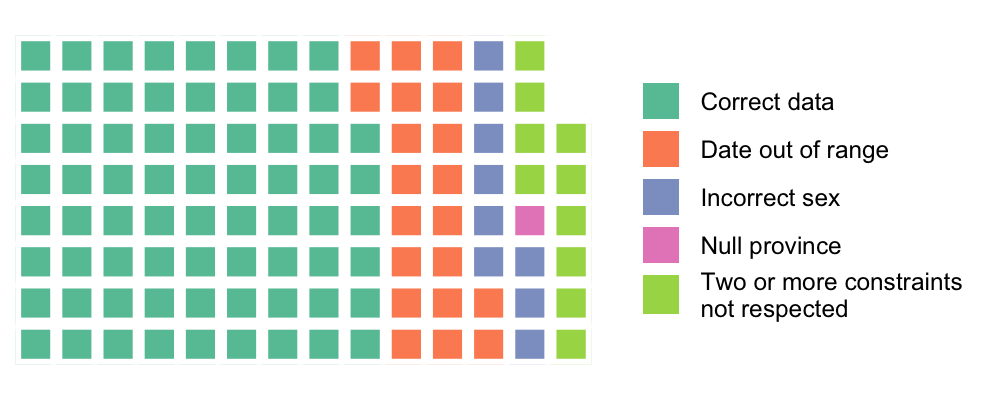
\includegraphics[scale=0.45]{../plots/patients-waffle.png}
	\caption{\small Information loss on patients, waffle plot}
	\label{waffle}
\end{figure}

There are no null provinces and birthdates. The bigger impact is caused by dates falling outside the acceptable range, meaning patients started treatment with their general practitioner earlier than 2000.

\subsection{\textit{diagnoses} (15 millions of tuples)}
\subsubsection{ICD-9}
An ICD-9 code is correct if it is present in the official ICD-9 database\cite{icd9}. General practitioners may use different formats and notations, so before removing codes each one has been subject to preprocessing and parsing.

An ICD-9 code is considered wrong if there is no match in the official DB after any of those transformations:
\begin{enumerate}
	\item Removal of the dot;
	\item Addition of 0 at the beginning;
	\item Addition of 0 at the end;
	\item Removal of the last 0.
\end{enumerate}

There are 76 distinct incorrect ICD-9 codes, a negligible amount considering the total records consisting in 9 895 distinct codes.

\subsubsection{Summary}
\begin{itemize}
	\item Incorrect ICD-9 codes: $76 \rightarrow 0.0005\%$;
	\item Null or empty ICD-9 codes: 2 103 169 $\rightarrow 13.02\%$;
	\item Null or empty descriptions: 656 067 $\rightarrow 4.24\%$;
	\item Dates out of range: 807 985 $\rightarrow 5.23\%$.
\end{itemize}

Empty descriptions almost always correspond to empty ICD-9 codes, therefore the total information loss on descriptions is absorbed by null codes, resulting in the same 13.02\% united percentage.

\subsection{\textit{prescriptions} (118 millions of tuples)}
\subsubsection{ATC code}
The ATC code, unlike ICD-9, has a univocal format (a numeric string of 7 digits), and no parsing is needed. All the codes have been checked with the ontologies in a well-known biology portal\cite{atc}, and an ATC is considered incorrect if there is no match.

There are 1 750 292 non-existent codes, which are caused by:
\begin{enumerate}
	\item Alteration of the codes within the years without updating the database;
	\item Single prescriptions indexed using the superclass code;
	\item Codes only recognised by local pharmacies.
\end{enumerate}

The latter is the most common reason: there are up to 90 000 occurrences of a single unofficial code. Those numbers, despite being high, are not majorly impacting results, considering the total amount of 118 millions of records.

\subsubsection{Summary}
\begin{itemize}
	\item Incorrect ATC codes: 1 750 292 $\rightarrow 1.47\%$;
	\item Null or empty ATC codes: 1 577 749 $\rightarrow 1.33\%$;
	\item Null or empty AIC codes: 1 310 719 $\rightarrow 1.1\%$;
	\item Null or empty descriptions: 101 248 410 $\rightarrow 85.28\%$;
	\item Dates out of range: 3 472 119 $\rightarrow 2.92\%$.
\end{itemize}

Clearly, the prescription description is not a field which can be used for reliable analytics since empty values prevail.

The field \textit{pieces} (number of boxes) might be useful to check for appropriate prescribing, but since the field is a string it requires casting and parsing to integer, and it could be more relevant to focus on prescription patterns.

\section{Total information loss}
Overall, total information loss is shown according by its belonging table. 

\begin{table}[!htb]
	
	\centering
	\begin{minipage}[c]{0.4\linewidth}
				\begin{tabular}{c|c|c}
				\textbf{Table} & \textbf{Records} & \textbf{Percentage} \\
				\hline
				\textit{patients} & 302 266 & 29\% \\
				\hline
				\textit{diagnoses} & 2 403 202 & 15.5\% \\
				\hline
				\textit{prescriptions} & 5 560 191 & 4.7\& \\
			\end{tabular}
	\end{minipage}
	\qquad
	\begin{minipage}[c]{0.4\linewidth}
		\qquad
		\centering
		$\rightarrow$
		\qquad
		\begin{tabular}{c}
			\textbf{Usable records} \\
			\hline
			713 352 \\
			\hline
			13 056 997 \\
			\hline
			113 156 212 \\
		\end{tabular}
		
	\end{minipage}
	\caption{\small Information loss summary}
\end{table}



The aggregated results are not final: each single output from interrogations will be influenced by all the different invalid fields (i.\ e. a patient could have all correct data yet a missing prescription AIC), creating a progressive deletion effect.

Overall, percentages do not compose the majority of tuples, since tables have magnitude order of millions.

